\documentclass[xcolor=table]{beamer}

\usepackage{pgf,pdfpages}
\usepackage{listings}
%\usepackage{adjustbox}
\usepackage{graphicx} % http://tex.stackexchange.com/questions/38177/including-large-tables-in-a-beamer-frame
\usepackage{booktabs}
\usepackage{tabularx}
\usepackage{array}

\usepackage[T1]{fontenc}
\usepackage{cmap}
\usepackage[utf8]{inputenc}

% syntax highlighting
\definecolor{sh_comment}{rgb}{0.12, 0.38, 0.18}
\definecolor{sh_keyword}{rgb}{0.37, 0.08, 0.25}
\definecolor{sh_string}{rgb}{0.06, 0.10, 0.98}

\lstset{
    language=C,
    numbers=left,
    numberstyle=\tiny,
    frame=tb,
    showstringspaces=false,
    captionpos=b,
    stringstyle=\color{sh_string},
    keywordstyle = \color{sh_keyword}\bfseries,
    commentstyle=\color{sh_comment}\itshape,
    basicstyle=\small\sffamily,
    numbersep=-5pt,
    belowskip=-\parskip,
    aboveskip=\baselineskip
}

%\lstset{breakatwhitespace,
%    language=C++,
%    columns=fullflexible,
%    keepspaces,
%    breaklines,
%    tabsize=3,
%    showstringspaces=false,
%extendedchars=true}

\mode<presentation>
{
    %\usetheme{bunsen}
    \usetheme{Madrid}
    \setbeamercovered{transparent}
    \setbeamertemplate{items}[circle]
}

\definecolor{lightgray}{gray}{0.9}
\definecolor{darkgreen}{RGB}{0, 150, 0}
\definecolor{darkred}{RGB}{150, 0, 0}
\definecolor{darkyellow}{RGB}{140, 140, 0}

% suppress navigation bar
\beamertemplatenavigationsymbolsempty

\usefonttheme[onlymath]{serif}
\setbeamerfont{frametitle}{size=\LARGE,series=\bfseries}

\defbeamertemplate{enumerate item}{mycircle}
{
    \begin{pgfpicture}{0ex}{0ex}{1.5ex}{0ex}
        \pgfbox[center,base]{\insertenumlabel.}
    \end{pgfpicture}
}
[action]
{\setbeamerfont{item projected}{size=\scriptsize}}
\setbeamertemplate{enumerate item}[mycircle]

%% SPACING BETWEEN ITEMS FOR BEAMER
%% following lets me add length between items
%% http://tex.stackexchange.com/questions/16793/global-setting-of-spacing-between-items-in-itemize-environment-for-beamer
% \let\oldframe\frame
% \renewcommand{\frame}{
% \oldframe
% \let\olditemize\itemize
% %%\renewcommand\itemize{\olditemize\addtolength{\itemsep}{0.5\baselineskip}}
% \renewcommand\itemize{\olditemize\addtolength{\parskip}{0.5\baselineskip}} %% this affects nested list (itemize) as well
% }
\newlength{\wideitemsep}
\setlength{\wideitemsep}{\itemsep}
\addtolength{\wideitemsep}{0.5\baselineskip}
\let\olditem\item
\renewcommand{\item}{\setlength{\itemsep}{\wideitemsep}\olditem}
%%\usepackage{enumitem} %% traditional way to modify listing (itemize and enumerate) properties...but beamer has its own definition
%% NESTED LISTS
%% http://tex.stackexchange.com/questions/20654/length-between-nested-lists
\setbeamertemplate{itemize/enumerate subbody begin}{\vspace{0.5\baselineskip}}
\setbeamertemplate{itemize/enumerate subbody end}{\vspace{0.5\baselineskip}}
%% MORE OPTIONS http://tex.stackexchange.com/questions/11168/change-bullet-style-formatting-in-beamer

\title{Sega Game Gear on a Chip}
\author{Max Thrun | Samir Silbak}
\institute{University of Cincinnati}
\date{Fall 2012}

\begin{document}

\maketitle

%
% background for the rest of the slides
%
%\setbeamertemplate{background}
%{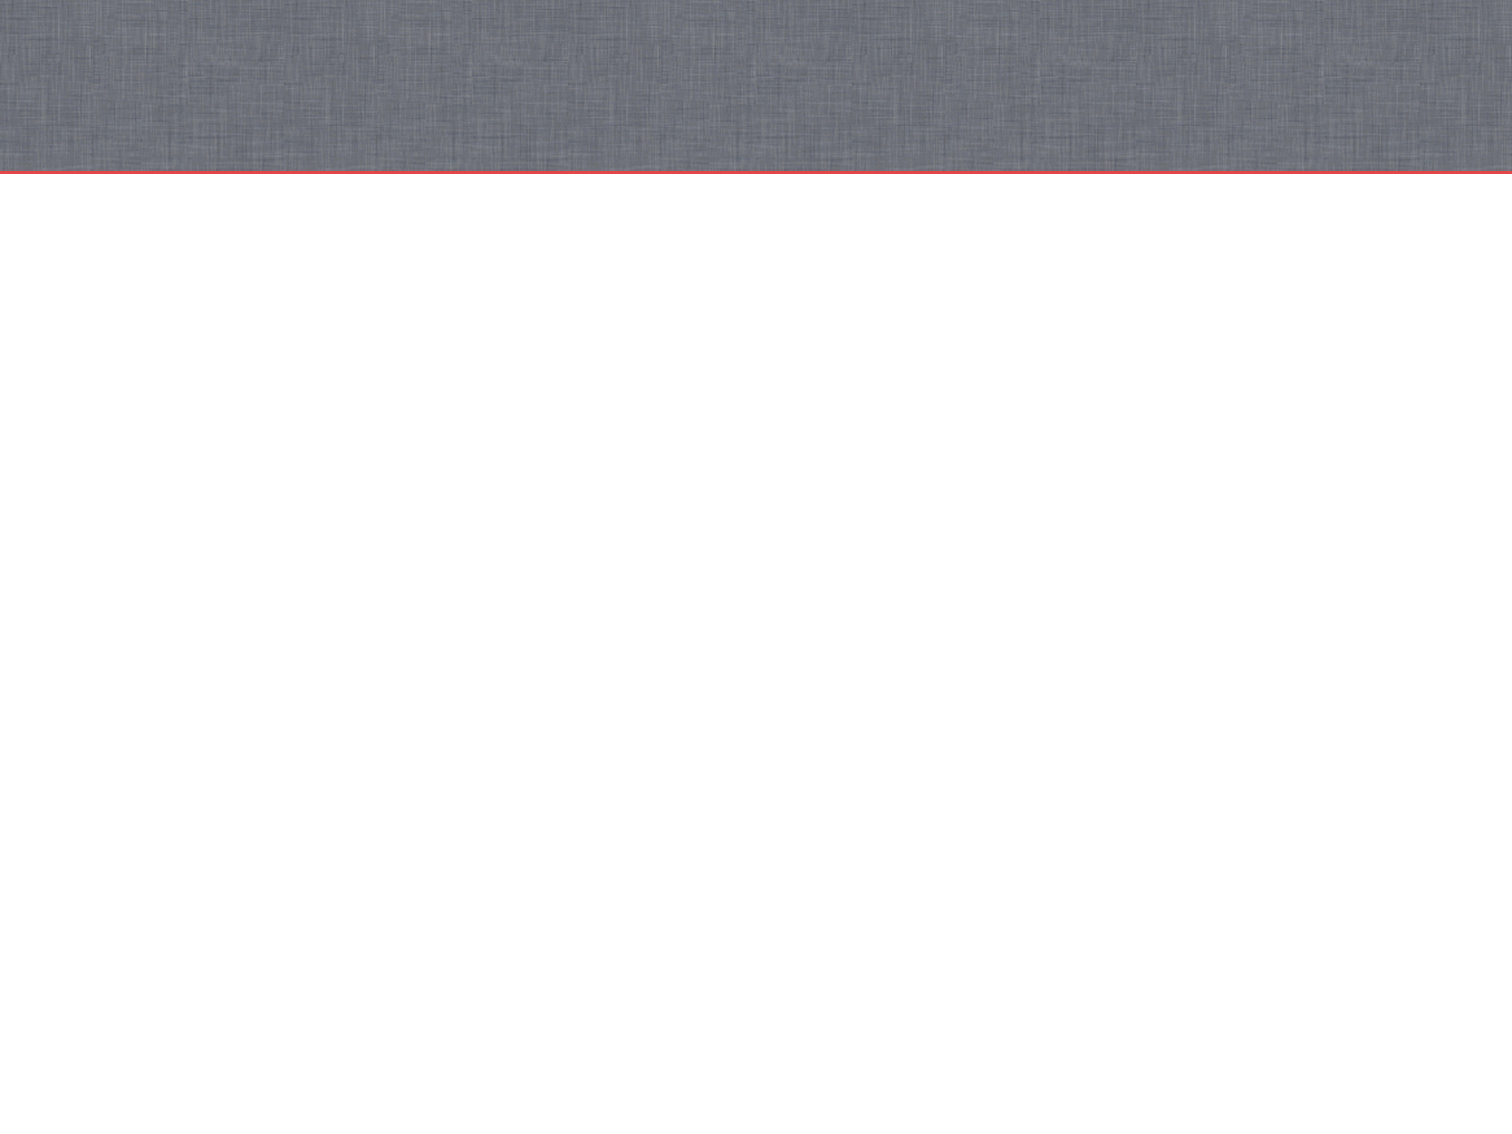
\includegraphics[width=\paperwidth,height=\paperheight]{slide_bg.png}}
%\setbeamertemplate{footline}[bunsentheme]

\begin{frame}
\frametitle{Agenda}
    \begin{itemize}
        \olditem Problem Description
        \olditem Design Process
        \olditem Implementation Priority
        \olditem Requirements
        \olditem Assessment Metrics
        \olditem Test Plans
        \olditem Design Overview
        \olditem Project Limitations
        \olditem Demonstration
    \end{itemize}
\end{frame}

\begin{frame}
    \frametitle{Problem Description}
    \begin{center}
        \Large
        Reimplement all the digital components of \\a legacy computer system in a FPGA
    \end{center}
\end{frame}

\begin{frame}
    \frametitle{Problem Description}

    \begin{columns}[c]
        \column{0.6\textwidth}
            Why?
            \begin{itemize}
                \item<2-> \textbf{Maintainability} - You can no longer buy parts to service legacy computer systems
                \item<3-> \textbf{Upgradability} - Reimplementation gives an opportunity to add additional features
                \item<4-> \textbf{Portability} - Do not need all the original big clunky hardware. Reimplementation can
                    be embedded in new designs
            \end{itemize}

        \column{0.4\textwidth}
            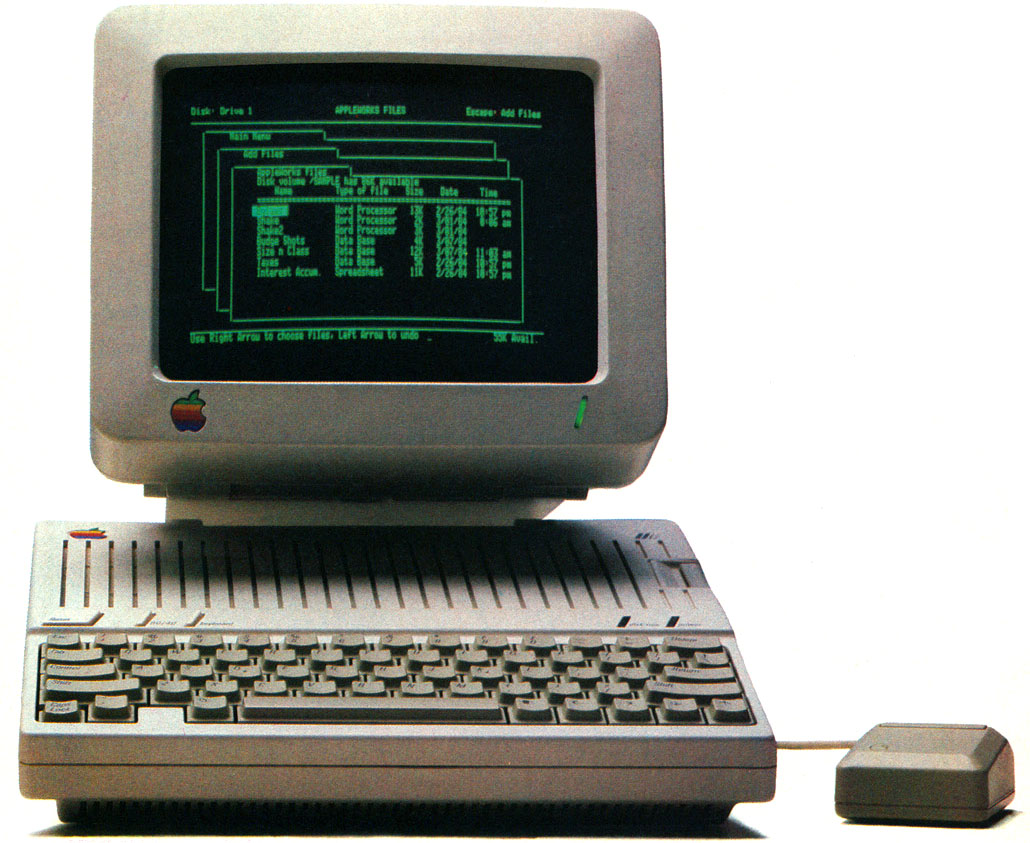
\includegraphics[width=\textwidth]{../images/apple_2.jpg}
    \end{columns}
\end{frame}

\begin{frame}
    \frametitle{Design Process}
    \begin{enumerate}
        \item<1-> Break down system components according to the original system architecture
        \item<2-> Implement each component in Verilog matching the original
            functionality described by official and non official documents
        \item<3-> Simulate each components functionality and compare it against the actual hardware (in our case an emulator)
        \item<4-> Tie components together in a way that is better suited toward FPGA technology (\emph{E.g.} avoid tri-state buses)
    \end{enumerate}
\end{frame}

\begin{frame}
    \frametitle{Implementation Priority}
    \begin{enumerate}
        \olditem Flash Memory Interface
        \olditem Memory Management Unit (MMU)
        \olditem Z80 + System RAM
        \olditem Cartridge Mapper
        \olditem VGA Driver
        \olditem Background Tiles + VRAM
        \olditem Video Display Processor Logic (VDP)
        \olditem Sprites
        \olditem Controller Input
        \olditem Sound
    \end{enumerate}
\end{frame}

\begin{frame}
    \frametitle{Requirements}
    \begin{enumerate}
        \item<1-> \textbf{VGA Output -} Need to output video via VGA which is
            the most common video interface found on FPGA development boards.
        \item<2-> \textbf{ROM Loading -} Need to be able to easily load in
            different game and test ROMs into the Flash memory chip on the dev
            board.
        \item<3-> \textbf{Accurate Re-implementation -} Overall goal of this
            project is to re-implement the Sega Game Gear as accurately as
            possible. User should not be able to tell its not the original
            hardware.
        \item<4-> \textbf{Accurate Architecture -} Overall system architecture
            should be as clean as possible and closely match that of the
            original Game Gear.
    \end{enumerate}
\end{frame}

\newcolumntype{L}[1]{>{\raggedright\let\newline\\\arraybackslash\hspace{0pt}}m{#1}}
\newcolumntype{C}[1]{>{\centering\let\newline\\\arraybackslash\hspace{0pt}}m{#1}}
\newcolumntype{R}[1]{>{\raggedleft\let\newline\\\arraybackslash\hspace{0pt}}m{#1}}
\begin{frame}
    \frametitle{Assessment Metrics}
    \rowcolors{1}{}{lightgray}
    \begin{tabular}{L{1in}L{1.9in}C{0.6in}C{0.7in}}
        \textbf{Function} & \textbf{Requirement Specification} & \textbf{Design Verified} & \textbf{Device Validated}\\
        \hline
        VGA Output               & Design must output video at 640x480 to a VGA monitor & {\color{darkgreen} Yes}     & {\color{darkgreen} Yes} \\
        Sega Mapper              & Design must implement the Sega Memory Mapper         & {\color{darkgreen} Yes}     & {\color{darkgreen} Yes} \\
        Video Display Processor  & Design must implement the TMS9918                    & {\color{darkyellow} Partly} & {\color{darkyellow} Partly} \\
        Game ROM stored in flash & Design must be able to load game ROMs from flash     & {\color{darkgreen} Yes}     & {\color{darkgreen} Yes} \\
        Controller Input         & Design must implement a single controller            & {\color{darkred} No}        & {\color{darkred} No} \\
        Game Gear system functionality & Design must implement the same functionality as the original Game Gear & {\color{darkyellow}Partly} & {\color{darkyellow}Partly} \\
        %\bottomrule
    \end{tabular}
\end{frame}

\begin{frame}
    \frametitle{Test Plans}
    Test plan split up into 4 areas:
    \vspace{\baselineskip}
    \begin{itemize}
        \item Z80, RAM, Cartridge
        \item VDP Background Tile Rendering
        \item System Simulation vs Emulator
        \item Custom test ROMs
    \end{itemize}
\end{frame}

\begin{frame}[fragile]
    \frametitle{Z80, RAM, Cartridge Test}
    Ensures basic code execution and memory/IO interfaces are working properly
    \vspace{\baselineskip}
    \begin{columns}[c]
        \column{0.55\textwidth}
        \begin{enumerate}
            \item Connect 8 LEDs to Z80 IO port 1
            \item Write simple Z80 test program that increments IO port 1
            \item Load test program into flash
            \item Divide Z80 clock down to 10Hz
            \item Verify LEDs incrementing on development board
        \end{enumerate}
        \column{0.45\textwidth}
        \begin{lstlisting}
  __sfr __at (0x01) debug;
  int main() {
      debug = 0x38;
      while (1) {}
      return 0;
  }
        \end{lstlisting}
    \end{columns}
\end{frame}

\begin{frame}
    \frametitle{VDP Background Tile Rendering Test}
    Ensures VDP background tile rendering works correctly without worrying about Z80 or interface logic
    \vspace{\baselineskip}
    \begin{columns}[c]
        \column{0.6\textwidth}
        \begin{enumerate}
            \item Obtain VRAM dump from the Osmose emulator
            \item Verify dump integrity using rendering program on computer
            \item Transfer dump to FPGA VRAM via the `MemSend' tool
            \item Verify that the resulting image on screen matches the emulator
        \end{enumerate}
        \column{0.4\textwidth}
        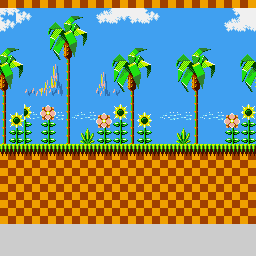
\includegraphics[width=\textwidth]{../images/screen.png}
    \end{columns}
\end{frame}

\begin{frame}
    \frametitle{System Simulation vs Emulator Test}
    Ensures that our system functionally matches a known good one
    \vspace{\baselineskip}
    \begin{enumerate}
        \item Insert print statements on all memory and IO accesses in emulator
        \item Do the same for the Verilog system level simulation
        \item Run emulator and simulation on same ROM
        \item Diff the print logs
        \item Verify that the memory and IO accesses match between the emulator
            and simulation
    \end{enumerate}
\end{frame}

\begin{frame}
    \frametitle{System Simulation vs Emulator}
    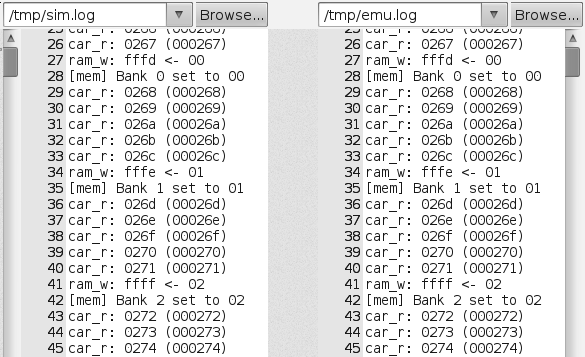
\includegraphics[width=\textwidth]{../images/diff_good.png}
\end{frame}

\begin{frame}
    \frametitle{System Simulation vs Emulator}
    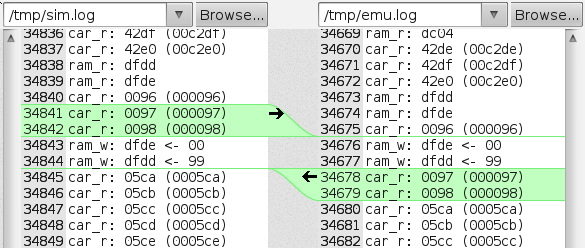
\includegraphics[width=\textwidth]{../images/diff_weird.png}
\end{frame}

\begin{frame}
    \frametitle{System Simulation vs Emulator}
    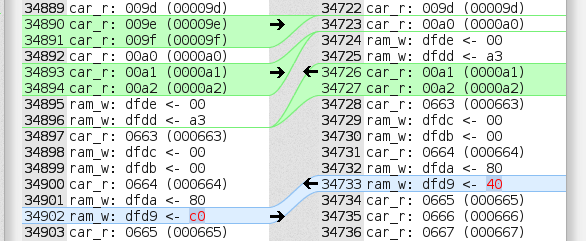
\includegraphics[width=\textwidth]{../images/diff_bad.png}
\end{frame}

\begin{frame}
    \frametitle{System Simulation vs Emulator}
    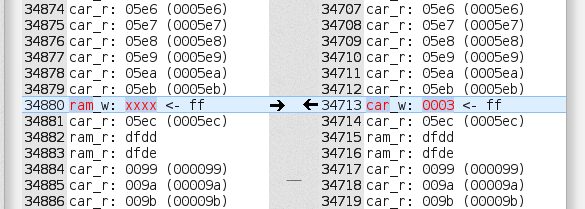
\includegraphics[width=\textwidth]{../images/diff_x.png}
\end{frame}

\begin{frame}
    \frametitle{Custom Test ROMs}
    Allows unit testing of specific features of the system
    \vspace{\baselineskip}
    \begin{columns}[c]
        \column{0.6\textwidth}
        \begin{enumerate}
            \item Write program that performs a certain task (ex. scroll screen left 5 pixels)
            \item Verify ROM in emulator
            \item Flash ROM onto the dev board
            \item Verify expected output is achived on FPGA
        \end{enumerate}
        \column{0.4\textwidth}
        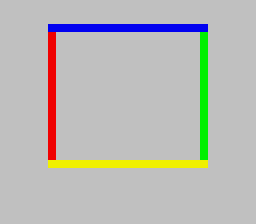
\includegraphics[width=\textwidth]{../images/scroll.png}
    \end{columns}
\end{frame}

\begin{frame}[fragile]
    \frametitle{Custom Test ROM Code Library}
    We ended up building a library of high level functions to quickly allow new tests to be written
    \begin{lstlisting}[basicstyle=\ttfamily\scriptsize]
  void vdp_write_control(uint8_t value);
  void vdp_write_data(uint8_t value);
  void vdp_set_register(uint8_t reg, uint8_t value);
  void vdp_set_vram_addr(uint16_t addr);
  void vdp_set_palette(uint8_t id, uint16_t color);
  void set_pattern_fill(uint16_t id, uint8_t color);
  void set_tile_to_pattern(uint8_t x, uint8_t y, uint16_t pattern);
  void delay(uint16_t x);
  void set_debug(uint8_t x);
    \end{lstlisting}
\end{frame}

\begin{frame}[fragile]
    \frametitle{Custom Test ROM Example}
    \begin{lstlisting}[basicstyle=\ttfamily\scriptsize]
    #include <stdint.h>
    #include <gg.h>

    int main() {
      uint8_t x = 0;

      while (1) {
          // set register 1 bit 6 to enable display
          vdp_set_register(1, (1<<6));

          // set color palette (0x0BGR)
          vdp_set_palette(0, 0x0CCC);     // gray
          vdp_set_palette(1, 0x000F);     // red
          vdp_set_palette(2, 0x00F0);     // green

          // update the debug leds
          set_debug(x++);
      }

      return 0;
    }
    \end{lstlisting}
\end{frame}

\begin{frame}
    \frametitle{Design Overview}
    \vspace{-0.5\baselineskip}
    \begin{center}
        Black Box Diagram \\
        \vspace{0.5\baselineskip}
        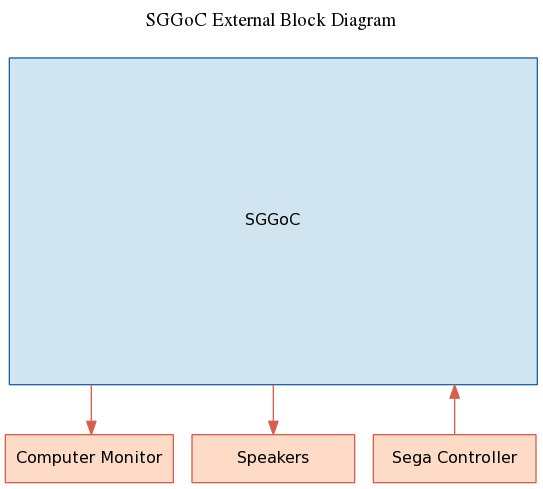
\includegraphics[scale=0.4]{../block_diagrams/block_diagram_external.png}
    \end{center}

\end{frame}

\begin{frame}
    \frametitle{Design Overview}
    \vspace{-0.5\baselineskip}
    \begin{center}
        Internal Functional Diagram \\
        \vspace{0.5\baselineskip}
        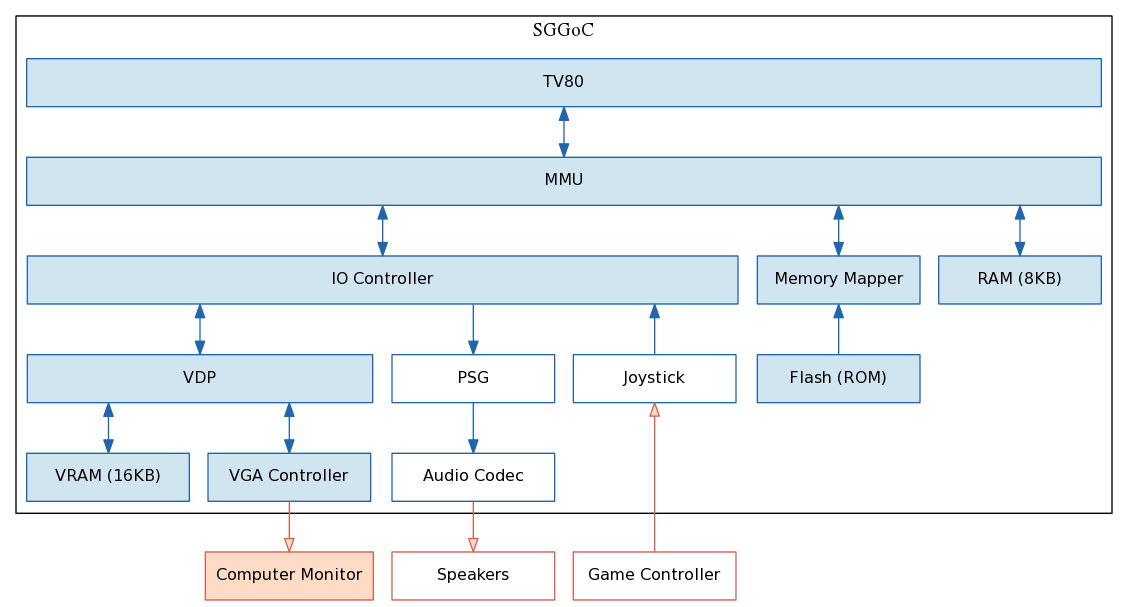
\includegraphics[scale=0.3]{../block_diagrams/block_diagram_internal_implemented.png}
    \end{center}
\end{frame}

\begin{frame}
    \frametitle{Design Overview}
    \begin{center}
        `Memsend' tool used to write ROMs to the flash chip on the FPGA development board
    \end{center}
    \begin{columns}[c]
        \column{0.45\textwidth}
        \begin{center}
            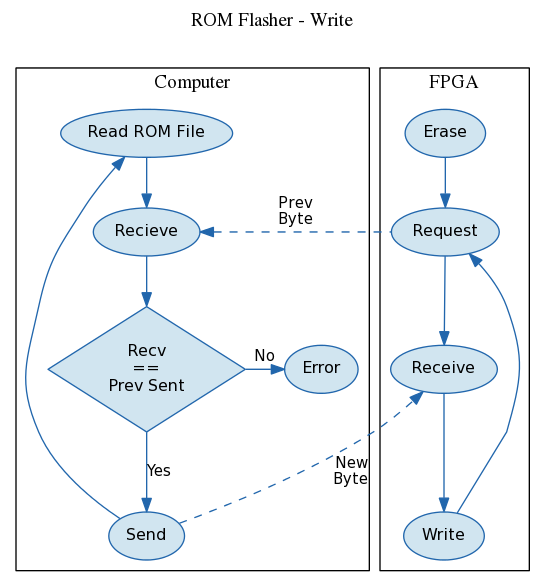
\includegraphics[width=\textwidth]{../../fpga/rom_flasher/doc/block_diagram_write.png} \\
            Write
        \end{center}
        \column{0.45\textwidth}
        \begin{center}
            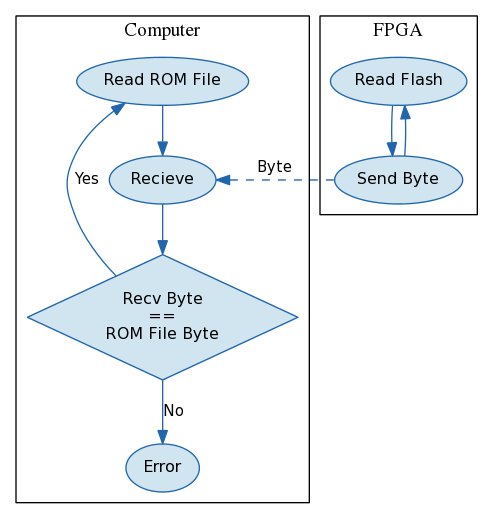
\includegraphics[width=\textwidth]{../../fpga/rom_flasher/doc/block_diagram_read.png} \\
            Read
        \end{center}
    \end{columns}
\end{frame}

\begin{frame}
    \frametitle{Project Limitations}
    \begin{itemize}
        \item<1-> \textbf{Tile Corruption - } Some tiles are fliped or are the
            wrong tile ID. Not sure if timing or logic issue yet. Haven't been
            able to reproduce with a test ROM yet.
        \item<2-> \textbf{Missing Features -} Currently missing some core
            functionality such as sprites, controller input, and sound. Each
            will be added with time.
        \item<3-> \textbf{Cumbersome ROM Loading -} The current process to load
            a new ROM is cumbersome and takes a long time. It can take 5-10
            minutes to flash a multi-megabyte ROM. Loading off an SD card would be
            much nicer.
    \end{itemize}
\end{frame}

\begin{frame}
    \frametitle{}
    \begin{center}
        \Huge
        Demonstration
    \end{center}
\end{frame}

\begin{frame}
    \frametitle{}
    \begin{center}
        \Huge
        Questions?
    \end{center}
\end{frame}

\newpage

\end{document}
